\documentclass[a4paper, 9pt, 
               xcolor={svgnames, dvipsnames},
               hyperref={colorlinks, linkcolor=myblue}]{beamer}
               
\definecolor{myblue}{RGB}{0,51,153}
%--------------------------------------------------------------------------%
%\usetheme{Boadilla}
%\usetheme{Singapore}
%\usecolortheme{dolphin}
\usetheme{Antibes}
%\usetheme{JuanLesPins}
%\usetheme{Singapore}
\usecolortheme{dove}
\usefonttheme{structurebold}
\setbeamertemplate{theorems}[numbered]
\setbeamertemplate{footline}[frame number]
\setbeamertemplate{navigation symbols}
   {\insertbackfindforwardnavigationsymbol}
   
   \setbeamertemplate{footline}
{
    \leavevmode%
    \hbox{%
        \begin{beamercolorbox}[wd=.25\paperwidth,ht=2.25ex,dp=1ex,center]{author in head/foot}%
            \usebeamerfont{author in head/foot}\insertshortauthor
        \end{beamercolorbox}%
        \begin{beamercolorbox}[wd=.7\paperwidth,ht=2.25ex,dp=1ex,right]{date in head/foot}%
            \usebeamerfont{date in head/foot}\insertshortdate{}\hspace*{2em}
            \insertframenumber{} / \inserttotalframenumber\hspace*{2ex} 
        \end{beamercolorbox}}%
        \vskip0pt%
}

\AtBeginSection[]{
	\begin{frame}
	\vfill
	\begin{center}
	\Huge\insertsectionhead\par%
	\end{center}
	\vfill
	\end{frame}
}
%--------------------------------------------------------------------------%
% Packages
\usepackage[hangul]{kotex}
\usepackage{mathpazo} % For graphics / images	
\usepackage{amsmath,amsfonts,amssymb,amsthm} % 수식으로 필수
\usepackage{booktabs}   % for table
\usepackage{color}
\DeclareMathOperator*{\argmin}{\operatorname{argmin}}
\newcommand{\R}{\mathbb{R}}
\newcommand{\e}{{\varepsilon}}
\newcommand{\E}{\mathbb{E}}
\newcommand {\for}{\quad\mbox{for}\quad}
\newcommand{\var}{{\rm Var}}
\newcommand{\m}{\mathsf}
\newcommand {\DOT}{{\, \cdot \, }}
\newcommand{\f}{\m{f}}
\newcommand{\s}{\m{s}}
\newcommand{\p}{\m{p}}
\newcommand {\fm}[1]{{\, \f \left( \DOT; #1 \right)}}
\newcommand {\sm}[1]{{\, \s \left( \DOT; #1 \right)}}
%\newcommand {\pm}[1]{{\, \p \left( \DOT; #1 \right)}}
\newcommand {\cm}[1]{{\, \m{c} \left( #1 \right)}}
\newcommand{\M}{\mathbb{M}}
\newcommand{\ed}{\end{document}}
\newcommand{\DB}[1]{\textcolor{Blue}{#1}}
\newcommand{\DR}[1]{\textcolor{DarkRed}{#1}}
\newcommand{\blue}[1]{{\color{blue} #1}}
\def\arraystretch{1.5}
%--------------------------------------------------------------------------%
% Title page
\title[Pliable Regression Splines]{Pliable regression splines with an auxiliary variable}
% \subtitle{Evaluation of a Master thesis}
\author{Jae-Kwon Oh}
\institute[Department of Information Statistics \\ Chungbuk National University]{ 
\includegraphics[scale = 0.4]{cbnulogo} \\ Department of Information Statistics \\ Chungbuk National University}
\date{2021. 5. 26.}


\begin{document}
\frame{\titlepage}

\section*{Contents}
\begin{frame}{Contents}
\tableofcontents
\end{frame}

% Section 1
\input{Introduction.tex}

% Section 2
\section{Pliable regression splines}
\begin{frame}{Bone mineral density data}
\begin{itemize}
\item 청소년과 젊은 성인들의 골밀도 (bone mineral density) 데이터
\end{itemize}
\begin{figure}
\includegraphics[scale=0.35]{BMD}
\end{figure}
\end{frame}

\begin{frame}{Nonparametric regression model}
\begin{itemize}
\item Data :
$$
(x_1, z_1, y_1), \ldots, (x_n, z_n, y_n)
$$
\vspace{3mm}
\item Model :
$$
y_i = \mathnormal{f}(x_i, z_i) + \varepsilon_i \quad \mbox{for} \quad i = 1, \ldots, n,
$$
where $y_i \in \mathbb{R}, \; x_i \in [0,1], \; z_i = (z_{i1}, \ldots, z_{iK}) \in \mathbb{R}^K, \; E(\varepsilon_i) = 0$ and $Var(\varepsilon_i) > 0$.
\vspace{3mm}
\item Goal : 
\begin{center}
Estimate $\mathnormal{f}$ based on the given data.
\end{center}
\end{itemize}
\end{frame}

\begin{frame}{Objective function}
\begin{itemize}
\item \blue{Pliable Spline Estimator (PSE)} :

For $x \in [0,1]$ and the binary vector $ z = (z_1, \ldots, z_K)$
with length $K$, define
% Linear combination of B-splines with auxiliary binary variable :
$$
f(x, z;\theta) = \sum_{j=1}^J \beta_j B_j(x) + \sum_{j=1}^J \sum_{k=1}^K \gamma_{jk} z_k B_j(x),
$$
where 
$\theta = (\beta, \gamma_1, \ldots, \gamma_J)$ is a coefficient vector with
$\beta = (\beta_1, \ldots, \beta_J) \in \R^J$ and
$\gamma_j = (\gamma_{j1}, \ldots, \gamma_{jK}) \in \R^K$
for $j = 1, \ldots, J$. 
\vspace{3mm}
\item Residual sum of squares objective function :
$$
R(\theta) = \frac{1}{2n}\sum_{i=1}^n (y_i - f(x_i, z_i;\theta))^2
$$
\end{itemize}
\end{frame}

\begin{frame}{Coordinate descent algorithm}
\begin{itemize}
\item Univariate objective function of $\beta_j$ and $\gamma_{jk}$ :
$$
r_j (\beta_j) = R(\tilde\beta^{(-j)},\tilde\gamma_1, \ldots, \tilde\gamma_J) 
$$
and
$$
r_{jk}(\gamma_{jk}) = R \left( \tilde\beta, \tilde\gamma_1, \ldots, \tilde\gamma_{j-1},
\tilde\gamma_j^{(-k)}, \tilde\gamma_{j+1}, \ldots, \tilde\gamma_J \right)
$$
\vspace{3mm}
\item Coordinate-wise update :
$$
\tilde\beta_j \leftarrow \argmin_{\beta_j \in \R} r_j(\beta_j)
\quad\mbox{and}\quad
\tilde\gamma_{jk} \leftarrow \argmin_{\gamma_{jk} \in \R} r_{jk}(\gamma_{jk}).
$$
\end{itemize}
\end{frame}

\begin{frame}{Update $\theta = (\beta_j, \gamma_j)$ by CDA}
\begin{itemize}
\item The quadratic form of $\beta_j$
$$
r_j(\beta_j) 
= \frac{\sum_{i=1}^n B_j^2(x_i)}{2n} \left ( \beta_j - 
\frac{\sum_{i=1}^n y_{ij} B_j(x_i)}{\sum_{i=1}^n B_j^2(x_i)} \right )^2 + (\mbox{terms independent for } \beta_j)
$$
\item Update $\beta_j$
$$
\tilde\beta_j \leftarrow \frac{\sum_{i=1}^n y_{ij} B_j(x_i)}{\sum_{i=1}^n B_j^2(x_i)} 
\for j = 1, \ldots, J.
$$
\item Similarly, $r_{jk}$ can be expressed as quadratic form of $\gamma_{jk}$
\iffalse
$$
r_{jk}(\gamma_{jk})
= \frac{\sum_{i=1}^n z_{ik}^2 B_j^2(x_i)}{2n} \left \{ \gamma_{jk} - 
\frac{\sum_{i=1}^n y_{ijk} z_{ik} B_j(x_i)}{\sum_{i=1}^n z_{ik}^2 B_j^2(x_i)} \right \}^2 
+ (\mbox{terms independent for } \gamma_{jk}) 
$$
\fi
\item Update $\gamma_{jk}$
$$
\tilde\gamma_{jk} \leftarrow \frac{\sum_{i=1}^n y_{ijk} z_{ik} B_j(x_i)}{\sum_{i=1}^n z_{ik}^2 B_j^2(x_i)} 
\for j = 1, \ldots, J, \; k = 1, \ldots, K.
$$
\end{itemize}
\end{frame}

% Section 3
\section{Numerical studies}
\iffalse %(1)
\subsection{Simulation}
\begin{frame}{Simulation}
비교 모델
\begin{itemize}
\item Regression Spline (RS)

보조변수 (auxiliary variable) 없이 B-spline basis의 선형 적합
\item Smoothing Spline (SS)

모든 예측변수에 대해 매듭 지정, smoothing 과 shrinkage 적용
\item Local Regression (LR) and Local Polynomial (LP)

 moving average, polynomial regression
\item 평가 기준 : MSE, MAE
$$
MSE(\hat{f}) = \frac{1}{n} \sum_{i = 1}^n (\hat{f}(x_i) - f(x_i))^2
\quad \mbox{and} \quad
MAE(\hat{f}) = \frac{1}{n} \sum_{i = 1}^n |\hat{f}(x_i) - f(x_i)|
$$
\end{itemize}
\end{frame}

\begin{frame}{Simulation -  Underlying function}
\begin{figure}
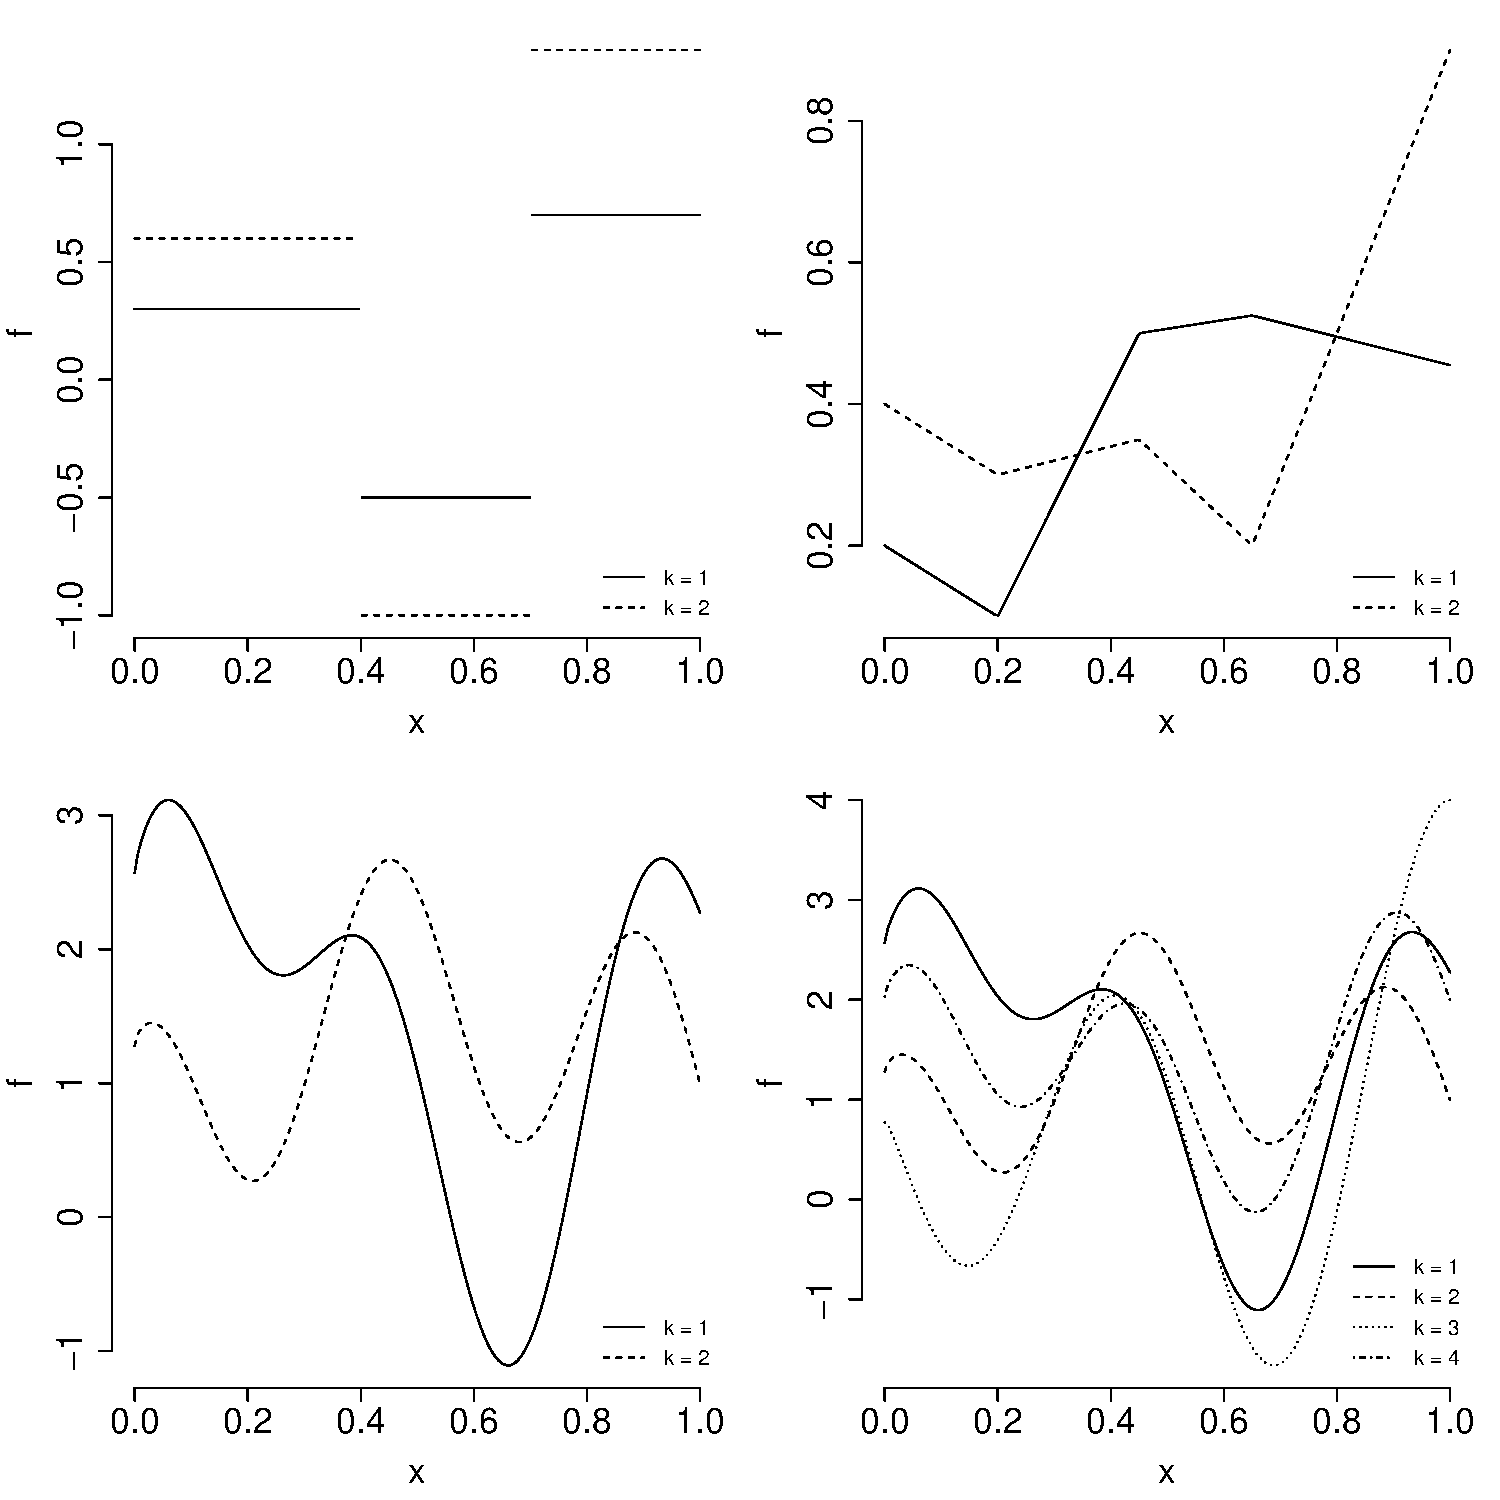
\includegraphics[scale = 0.28]{true_function}
\end{figure}
\end{frame}

\begin{frame}{Simulation - Results}
\begin{table}[!htb]
\centering
\footnotesize
\caption{The average of each criterion ($\times 100$) over $100$ runs of OUR, RS,
SS, LR, and LP for Example 1 with a sample size $n = 200, 500$ and a signal-to-noise ratio 
$SNR = 5, 15$, with the standard error in parentheses. The bold text is the smallest
criterion in each scenario.}
\label{tb : ex1}
\tabcolsep=5pt
\begin{tabular}{lllll||lllll}
  \hline
$n$ & SNR & Method & MSE & MAE & $n$ & SNR & Method & MSE & MAE \\ 
  \hline
200 & 5 & PSE & \textbf{2.86(1e-03)} & \textbf{8.77(2e-03)} & 500 & 5 & PSE & \textbf{2.13(5e-04)} & \textbf{5.88(1e-03)} \\ 
   &  & RS & 8.96(6e-04) & 25.29(8e-04) &  &  & RS & 8.31(3e-04) & 25.20(3e-04) \\ 
   &  & SS & 4.02(7e-04) & 13.96(1e-03) &  &  & SS & 2.52(3e-04) & 10.65(1e-03) \\ 
   &  & LR & 13.93(1e-03) & 26.07(1e-03) &  &  & LR & 14.10(8e-04) & 26.01(8e-04) \\ 
   &  & LP & 11.86(8e-03) & 18.16(4e-03) &  &  & LP & 6.57(3e-03) & 12.54(2e-03) \\  \cline{2-5} \cline{7-10}
   & 15 & PSE & \textbf{1.79(7e-04)} & \textbf{5.52(1e-03)} &  & 15 & PSE & 1.68(5e-04) & \textbf{3.83(7e-04)} \\ 
   &  & RS & 8.34(6e-04) & 25.20(6e-04) &  &  & RS & 8.06(3e-04) & 25.16(3e-04) \\ 
   &  & SS & 2.15(4e-04) & 9.57(8e-04) &  &  & SS & \textbf{1.35(2e-04)} & 7.48(5e-04) \\ 
   &  & LR & 13.72(1e-03) & 25.47(1e-03) &  &  & LR & 13.74(8e-04) & 25.40(7e-04) \\ 
   &  & LP & 9.58(7e-03) & 13.98(4e-03) &  &  & LP & 6.11(3e-03) & 9.78(2e-03) \\ 
   \hline
\end{tabular}
\end{table}
\end{frame}

\begin{frame}{Simulation - Results}

\end{frame}
\fi %(1)

\subsection{Real data}
\begin{frame}{Bone mineral density data}
\begin{itemize}
\item 성별에 따라 골밀도의 분포가 다름
\end{itemize}
\begin{figure}
\includegraphics[scale=0.35]{BMD}
\end{figure}
\end{frame}

\begin{frame}{Bone mineral density data}
\begin{itemize}
\item 인종에 따라 골밀도의 분포가 다름
\end{itemize}
\begin{figure}
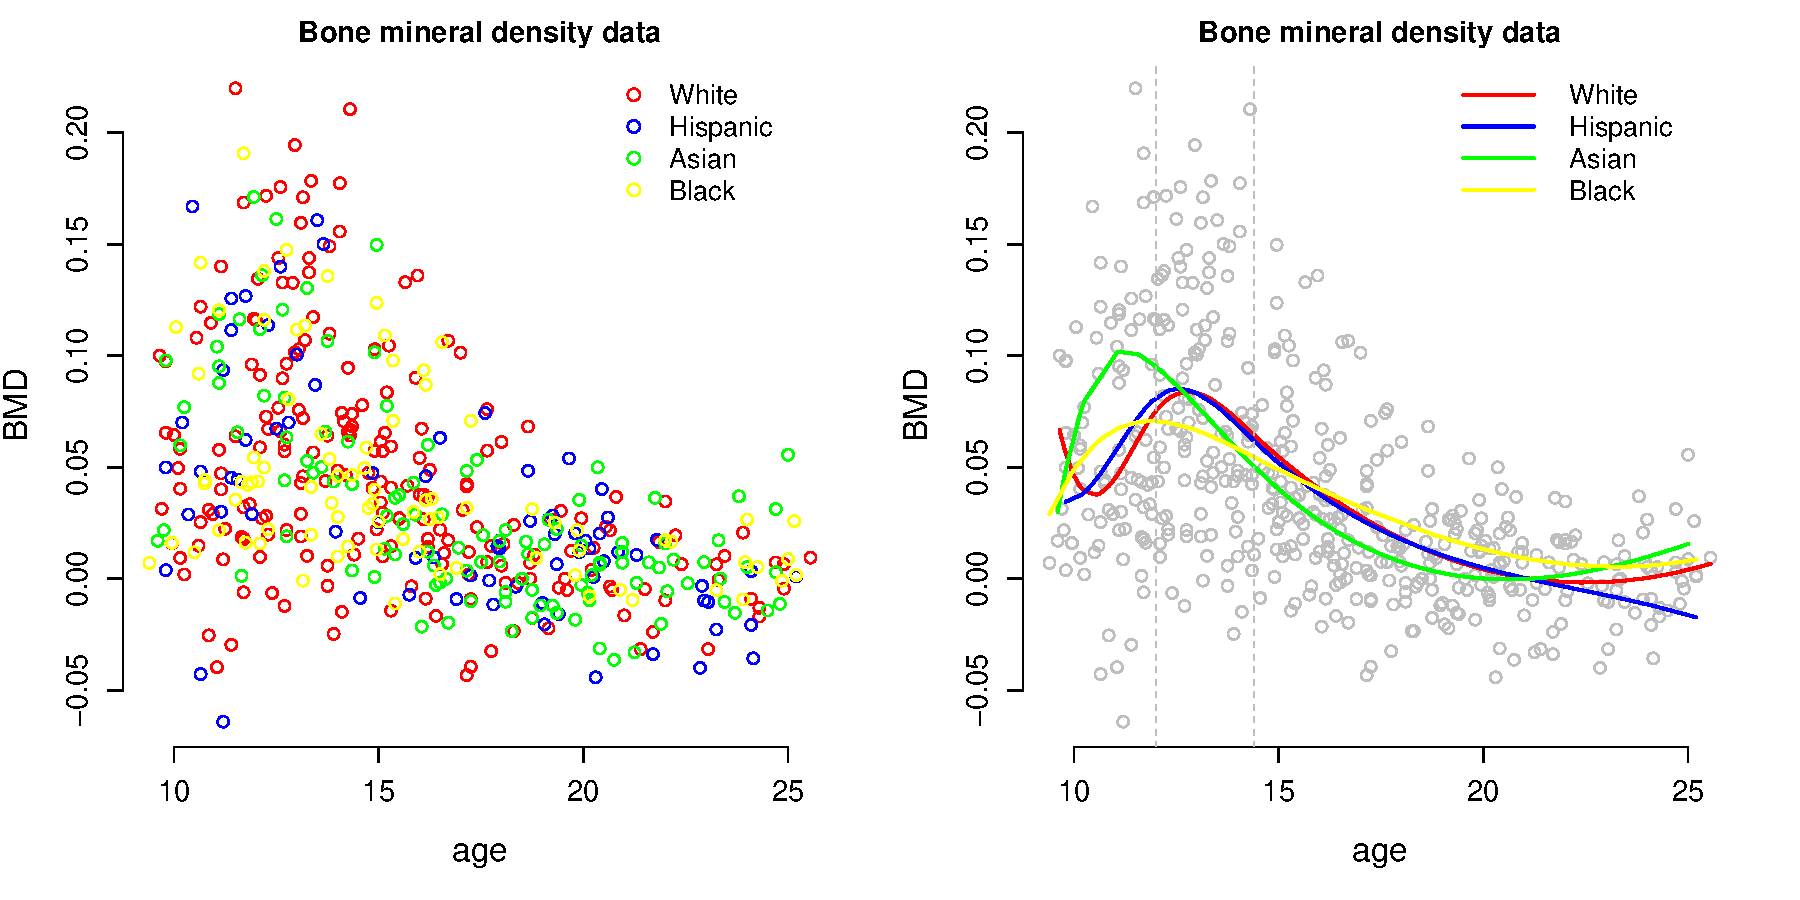
\includegraphics[scale=0.35]{BMD_e}
\end{figure}
\end{frame}

\begin{frame}
\begin{figure}
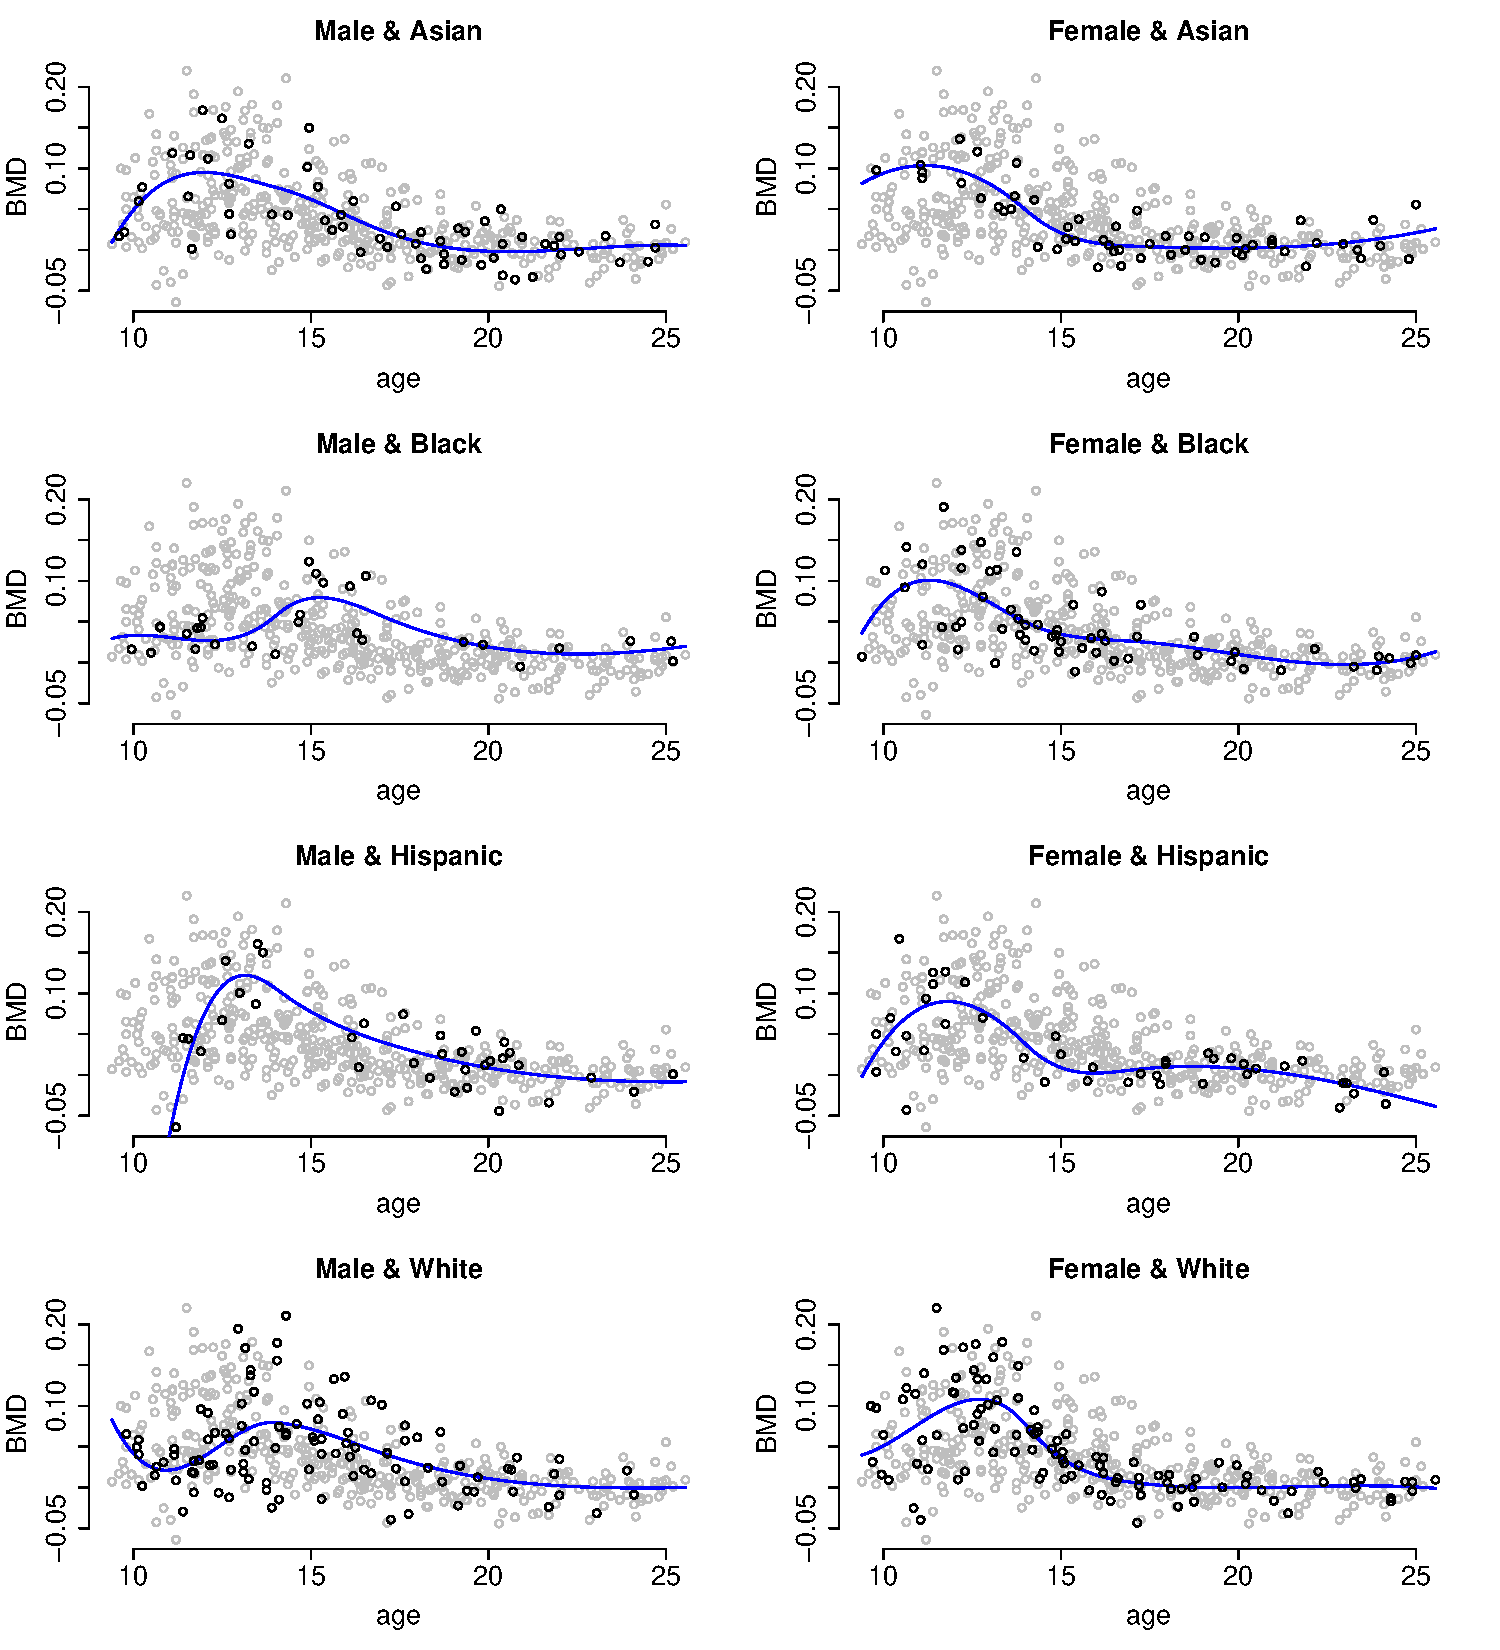
\includegraphics[scale=0.3]{gridz8_blue}
\end{figure}
\end{frame}


% Section 4
\section{Conclusion}
\begin{frame}{Conclusion}
\begin{itemize}
\item 비모수 함수 추정에서 B-spline을 사용하여 예측변수 외에 보조변수 (auxiliary variable) 가 추가된 경우에 적합한 Pliable Spline Estimator 제시
\vspace{3mm}
\item Coordinate descent algorithm 으로 목적함수를 최소화
\vspace{3mm}
\item 매듭 선택으로 단계적 선택법을 도입으로 최적의 knots 선택
\vspace{3mm}
\item 시뮬레이션과 실 데이터 분석을 통해 제안한 모델의 성능 확인
\end{itemize}
\end{frame}

\iffalse %(1)
% Section 5
\section{Discussion}
\begin{frame}{Discussion}
\begin{itemize}
\item Nonparametric quantile regression function estimator
\item addition of an appropriate penalty term for knot selection 
\end{itemize}
\end{frame}
\fi %(1)

\end{document}
